\documentclass[11pt,a4paper]{article}
\usepackage[margin=2.5cm]{geometry}
\usepackage[T1]{fontenc}
\usepackage{lmodern}
\usepackage{amsmath}
\usepackage{booktabs}
\usepackage{graphicx}
\usepackage{tabularx}
\usepackage{array}
\usepackage[round]{natbib}
\usepackage{xurl}
\usepackage[hidelinks]{hyperref}
\usepackage{setspace}
\setstretch{1.15}

\makeatletter\newcommand{\tabin}[1]{\@@input #1 }\makeatother
\newcommand{\gap}{40}
\newcommand{\nvshare}{83}
\newcommand{\nvsharesmh}{80}
\newcommand{\coren}{4}


\title{How much of Nvidia can academia explain?\\ Testing theories of CEO scandal on the 2026 episode\\ and on 79 earlier cases}
\author{Xiangzhong (Shaun) Meng\thanks{Independent researcher. Data: CRSP, Compustat, ExecuComp and RavenPack (Dow Jones edition) through WRDS; the open CEO dismissal database of \citet{gentry2021}; daily and hourly prices from Yahoo Finance for 2026. All errors are mine.}}
\date{November 2026\\[2pt] \small Working paper. Comments welcome.}

\begin{document}
\maketitle

\begin{abstract}
\noindent In October and November 2026 Nvidia's co-founder and chief executive went, in ten trading days, from the subject of a newspaper report to a former chief executive. Over the same period Nvidia's share price fell by about a fifth relative to the market and to its largest peers. I take eight predictions from research on executive misconduct, chief executive turnover, disclosed investigations, founders, board control and after-hours trading, and I test each prediction against Nvidia's abnormal returns before the open, during regular trading and after the close. I then test the same predictions on 79 personal-conduct scandals involving the chief executives of US listed companies from 2000 to 2024. Six predictions hold for Nvidia, one cannot yet be tested and one fails. The failed prediction is the size and timing of the first loss: the first newspaper report was followed by an abnormal return of about $-1$\%, and the board's announcement of an investigation ten days later by $-13.3$\% over two trading days. On a close-to-close basis Nvidia's share price fell again on the day the resignation was announced. Split by trading session, that fall took place on the previous evening, after new allegations were published, and from the last trade that evening the resignation day brought a rise of 3.8\%. In seven of the eight earlier cases in which an allegation became public before the chief executive left, the share price also rose at the departure. During the episode 69\% of Nvidia's abnormal price movement took place outside regular trading hours, against 26--36\% in the two months before.

\medskip\noindent\textit{JEL codes:} G14, G34, M12. \quad \textit{Keywords:} key-person risk, CEO misconduct, event study, disclosure, founder CEOs, after-hours trading, Nvidia.
\end{abstract}

\section{Introduction}

On 29 October 2026 a newspaper reported that Jensen Huang, the co-founder and chief executive of Nvidia, had had a close relationship with an executive of one of the company's cloud customers, and that this executive was under scrutiny by US officials. The company replied that meetings with customers were part of a chief executive's job \citep{techcrunch2026timeline}. On Sunday 8 November Nvidia's board announced an independent investigation, and on the same day Mr Huang wrote to the company's staff that he had been unfaithful to his wife \citep{nvidia2026message}. On the evening of 11 November further reports described a relationship with an employee who reported directly to him. The board accepted his resignation that day, and the company announced it before the market opened on 12 November \citep{nvidia2026eightk}. On 17 November Mr Huang said that he would be honoured to return if the board wanted him, and that evening the board's chair said that the board did not intend to reinstate him \citep{cnbc2026nov17,ft2026huang,techcrunch2026nov17}. Before the first report Nvidia was worth about \$5.2 trillion. Between the first report and 17 November its share price fell by 20.7\% relative to the market and the six other largest US technology companies.

Research in finance has studied most elements of this episode separately. \citet{cline2018} find that shareholders lose 4.1\% over three days when news of a chief executive's personal indiscretion first breaks. \citet{borelli2021} find that sexual-harassment scandals reduce company value by about 1.5\% over two days, and by a further 5.1 percentage points when the chief executive is involved. \citet{huson2004} find that forced departures of chief executives in which an outsider takes over are followed by a positive abnormal return of 2.1\%. \citet{blackburne2021} find that only 19\% of investigations by the Securities and Exchange Commission are disclosed when they begin. \citet{adams2005} find that companies run by founders who keep the chief executive title have more variable performance, and \citet{fahlenbrach2009} finds that they are valued more highly. \citet{barclay2003} find that trading outside regular hours produces significant price discovery, but at less efficient prices than regular trading. Each of these findings implies something about what Nvidia's share price should have done, and this paper turns each of them into a prediction and tests it.

I test the predictions in two ways. The first test uses Nvidia's abnormal returns, which I split into the pre-market session, regular trading and the after-hours session on each day. The second test uses 79 personal-conduct scandals involving the chief executives of US listed companies from 2000 to 2024, which I take from the dismissals for misconduct in the open turnover database of \citet{gentry2021} and from Dow Jones news stories that name a sitting chief executive together with words such as allegation, harassment or probe. I sort these cases by the order in which the market learned of them. In one-stage cases the misconduct became public on the same day as the chief executive's departure. In two-stage cases, which resemble Nvidia, an allegation or a board investigation became public first and the departure followed later. In survival cases the chief executive was still in office a year after the allegation.

Six of the eight predictions hold for Nvidia. The first newspaper report about the chief executive's private life was followed by a small abnormal return. The board's announcement of an investigation was followed by the largest abnormal return of the episode. The total loss was large. Once the trading sessions are separated, the resignation day shows a rise in the share price. The board refused the former chief executive's offer to return, and he controlled 3.6\% of the votes. Most of the abnormal price movement took place outside regular trading hours. The prediction that customers penalise a company whose leader is caught up in a scandal cannot yet be tested, because the only evidence so far is one revenue forecast.

The prediction that fails concerns the first loss. The literature puts it at about 4\% when the news first breaks. At Nvidia the first report was followed by an abnormal return of about $-1$\%, and the board's announcement ten days later by $-13.3$\% over two trading days, or about \$600 billion.

The session split changes one conclusion. On a close-to-close basis, Nvidia's abnormal return on the day the resignation was announced was $-3.5$\%. The allegations of 11 November were published after the close, and in after-hours trading that evening the abnormal return was $-7.0$\%. From the last trade that evening to the end of 12 November, the abnormal return was $+3.8$\%: $-5.4$\% before the open and $+8.8$\% during regular trading. In seven of the eight earlier two-stage cases the share price also rose when the chief executive left. Over the episode as a whole, 69\% of Nvidia's abnormal price movement took place outside regular hours, compared with 26\% and 36\% in the two months before.

\section{What happened at Nvidia}\label{sec:nvidia}

Throughout the paper, an abnormal return is the part of a share's return that its benchmark does not explain. For Nvidia the benchmark combines the S\&P~500 index fund SPY and an equal-weighted basket of the six other largest US technology companies: Apple, Microsoft, Alphabet, Amazon, Meta and Tesla. The weights on SPY and the basket come from a regression of Nvidia's daily returns on theirs over 250 trading days that end 81 trading days before 29 October. The benchmark absorbs movements of the whole market and of the technology sector, such as the fall in the market on 5 November. The semiconductor fund SMH is not the main benchmark, because Nvidia is one of its largest holdings; Table~\ref{tab:nvidia} reports it, together with a model that uses the market alone, as a check. Prices are daily closing prices from Yahoo Finance up to the close of 17 November 2026.

The first report was published at 5:01 am on 29 October, before the market opened. Over that day and the next, Nvidia's abnormal return was $-1.1$\%. Over the following three trading days, which came after a Saturday report on the concerns of intelligence officials about the customer executive, it was $-4.5$\%. The request from three House committee chairs for a closed-door briefing and a report on a US government memo were followed by an abnormal return close to zero. The board announced its investigation on Sunday 8 November, and Mr Huang's email to staff was released on the same day. Over the next two trading days Nvidia's abnormal return was $-13.3$\% (standard error 2.4), and the other two benchmarks give almost the same figure. On 11 November the shares moved with the market until the close. The reports of a relationship with a direct report appeared that evening, and in after-hours trading the shares fell by about 8\%. The board accepted the resignation on the same day, and before the market opened on 12 November the company filed the announcement with the Securities and Exchange Commission \citep{nvidia2026eightk}. The filing named the chief financial officer as interim chief executive and appointed the company's first chair. The close-to-close abnormal return of 12 November, $-3.5$\%, includes the after-hours trading of the evening before. Of the abnormal fall between 29 October and 12 November, \nvshare\% took place before 12 November, or \nvsharesmh\% with SMH as the benchmark.

On Friday 13 November a representative of the board said that it was choosing a search firm to find a successor. Shortly after noon on Monday 16 November, CNBC reported that the board was not considering bringing Mr Huang back and that it had hired a law firm to lead its investigation into his conduct and into whether national security or company secrets had been compromised \citep{cnbc2026nov16}. Nvidia's abnormal return that day was $-0.5$\%. On Tuesday 17 November, during trading hours, Mr Huang said in a statement that if the board decided that his return was in the interest of shareholders, employees, the company and America, he would be honoured to return as chief executive \citep{cnbc2026nov17}. The Financial Times reported that he also said he had made serious mistakes in his personal life and would co-operate with the investigation, that some technology executives and shareholders were campaigning for his return, and that the US President had said he was open to it \citep{ft2026huang}. A few days earlier the President had suggested Apple's chief executive as a possible successor \citep{fox2026cook}. Nvidia's abnormal return that day was $+1.6$\%. On the same day the board set up a committee to oversee the company's compliance with national security and export controls \citep{nvidia2026committee}.

After the market closed on 17 November, Nvidia reported revenue of \$115.8 billion for the quarter that ended on 25 October, 103\% more than a year earlier, and forecast revenue of about \$130 billion for the following quarter. The forecast assumes no sales of data-centre computing products in China \citep{nvidia2026q3}. The results release referred to the investigation as ``the ongoing investigation by an independent committee'' of the board, and it listed the change of leadership and the search for a new chief executive among the risks to the company's forecasts. On the call with analysts that evening, the chair, Harvey Jones, said that ``the Nvidia board unanimously accepted his resignation and does not intend to reinstate Jensen as CEO'', and that the board was considering both internal and external candidates \citep{techcrunch2026nov17}. The interim chief executive, Colette Kress, said that the business was continuing as usual, and in after-hours trading the shares rose by more than 3\% \citep{cnbc2026nov17earnings}.

\begin{table}[t]\centering\small
\caption{Nvidia, October--November 2026: abnormal returns by news date (\%)}\label{tab:nvidia}
\footnotesize\setlength{\tabcolsep}{4pt}
\begin{tabular}{>{\raggedright\arraybackslash}p{6.3cm}rrrr}\toprule
 & \multicolumn{2}{c}{Market and mega-cap basket} & Market and SMH & Market only \\
Trading days: news & CAR & (SE) & CAR & CAR \\ \midrule
\tabin{tables/t_nvidia.tex}
\bottomrule\end{tabular}
\par\medskip\footnotesize Cumulative abnormal returns (CAR) from daily closing prices from Yahoo Finance up to 17 November 2026, with standard errors in parentheses. Market: SPY. Basket: equal-weighted Apple, Microsoft, Alphabet, Amazon, Meta and Tesla. One estimation window of 250 trading days ending 81 trading days before 29 October. Event times come from SEC filings and the publishers' pages (events/nvidia\_timeline\_sources.csv).
\end{table}

\subsection{Abnormal returns by trading session}\label{sec:sessions}

The first report appeared at 5:01 am, the board's statement on a Sunday, the reports of 11 November after the close, the resignation before the open, and the quarterly results after the close. A daily closing price combines each of these with everything else that happened before the next close. I therefore split each trading day into three sessions, using daily and hourly prices from Yahoo Finance that include trading outside regular hours. The pre-market session runs from the last trade of the previous evening to the official opening price. Regular trading runs from the open to the official close. The after-hours session runs from the close to the last trade of the evening. In each session, Nvidia's abnormal return is its return minus the returns of SPY and of the peer basket in the same session, each multiplied by the weight estimated from daily returns. Yahoo reports no trading volume outside regular hours, so volume is compared by day.

Table~\ref{tab:sessions} compares three periods: the second month before the first report, the month immediately before it, and the episode. The measure is the weighted price contribution of \citet{barclay1993}, who use it to measure the share of a stock's cumulative price change that takes place in trades of a given size; \citet{barclay2003} use the same measure to compare trading sessions. It gives the share of a period's price movement that takes place in each session, with each day weighted by the size of its movement. In the two months before the first report, regular trading accounted for 64\% and 74\% of Nvidia's abnormal price movement. During the episode it accounted for 31\%, the pre-market session for 44\% and the after-hours session for 26\%. Over the same periods, the share of the peer basket's own movement outside regular hours stayed between 34\% and 43\%. Nvidia's mean absolute abnormal return was about 100 basis points a day before the episode and 327 basis points during it, and its daily trading volume during the episode was 2.6 times its level two months earlier.

Table~\ref{tab:sessiondays} shows each session on the days with news. On 9 November, the first trading day after the board's Sunday announcement, the abnormal return was $-9.6$\% before the open and $+0.4$\% during regular trading. On 11 November the abnormal return in after-hours trading, after the reports of a relationship with a direct report, was $-7.0$\%. The resignation was filed at 8:52 am on 12 November. The abnormal return was $-5.4$\% before the open, with most of the fall in the last half hour before the opening bell, and $+8.8$\% during regular trading, with most of the rise in the first hour. On 16 November the report that the board would not take Mr Huang back was published at 12:38 pm, and the abnormal return in regular trading that day was slightly positive. On 17 November the abnormal return in regular trading, the session in which Mr Huang made his offer to return, was $+0.6$\%, and in after-hours trading, after the results and the chair's statement, it was $+3.4$\%.

\begin{table}[t]\centering\small
\caption{Nvidia: shares of abnormal price movement by trading session, before and during the episode}\label{tab:sessions}
\scriptsize\setlength{\tabcolsep}{3pt}
\begin{tabular}{>{\raggedright\arraybackslash}p{3.2cm}rcccccrr}\toprule
 & & \multicolumn{4}{c}{Nvidia, abnormal: share (\%)} & Peers: & Mean $|$move$|$ & Volume \\ \cmidrule(lr){3-6}
Period & Days & Pre-market & Regular & After & Outside & outside (\%) & (bp a day) & ($\times$) \\ \midrule
\tabin{tables/t_sessions.tex}
\bottomrule\end{tabular}
\par\medskip\footnotesize Share: weighted price contribution, $\sum_t \mathrm{sign}(r_t)\, r_{s,t} / \sum_t |r_t|$, where $r_{s,t}$ is the log return in session $s$ on day $t$ and $r_t$ is the day's total. ``Outside'' is the pre-market and after-hours sessions together. Abnormal: Nvidia's session return minus its weights on SPY and on the peer basket (Apple, Microsoft, Alphabet, Amazon, Meta, Tesla) times their session returns. Peers: the share of the equal-weighted basket's own movement outside regular hours. Mean $|$move$|$: the mean absolute abnormal return per day. Volume: Nvidia's daily volume relative to the first period. Daily and hourly prices from Yahoo Finance.
\end{table}

\begin{table}[t]\centering\scriptsize
\caption{Nvidia: abnormal return by trading session on the days with news (\%)}\label{tab:sessiondays}
\setlength{\tabcolsep}{3pt}
\begin{tabularx}{\textwidth}{l>{\raggedright\arraybackslash}Xrrrrr}\toprule
Day & News & Pre-market & Regular & After-hours & Day & Volume ($\times$) \\ \midrule
\tabin{tables/t_session_days.tex}
\bottomrule\end{tabularx}
\par\medskip\footnotesize Log returns. The pre-market session runs from the last after-hours trade of the previous day to the open, so the ``Day'' column runs from the previous evening to the evening of the day shown and differs from the close-to-close returns in Table~\ref{tab:nvidia}. Times are US Eastern.
\end{table}

\section{Eight predictions, tested on Nvidia}\label{sec:theories}

\subsection{An accounting of the price response}\label{sec:frame}

The accounting below ignores the compensation that investors require for bearing risk and assumes that investors learn nothing between announcements beyond what the announcements contain. Once an allegation about a chief executive is public, the company faces three kinds of cost. Some costs fall on the company whatever the board decides: lawsuits, inquiries by regulators, the cost of the investigation, and damage to the company's reputation that a departure would not repair. I denote these costs by $c$. If the chief executive leaves, the company loses what that person contributed, together with the cost and the risk of finding a successor; I call this the key-person loss and denote it by $K$. If the chief executive stays, the company bears continuing damage to its reputation, the distraction of a leader under attack, the risk of further revelations and possible reactions from regulators or customers; I denote this cost by $D$. Investors judge that the chief executive will leave with probability $p$. All three costs are measured as a share of the company's value.

When the allegation becomes public, the share price falls by the expected cost:
\begin{equation}
R_{\text{first}} = -\bigl[\,c + pK + (1-p)D\,\bigr].
\end{equation}
When the board announces the departure, the company bears $K$ with certainty, and the price moves by
\begin{equation}
R_{\text{exit}} = (1-p)\,(D - K).
\end{equation}
A rise in the share price at the departure therefore corresponds to $D$ larger than $K$: investors judged that keeping the chief executive would have cost the company more than losing that person. A fall corresponds to $K$ larger than $D$. The sum of the two movements is
\begin{equation}
R_{\text{first}} + R_{\text{exit}} = -(c + K),
\end{equation}
the cost of the scandal to the company after the chief executive has gone. A one-stage case measures the same quantity in a single announcement. News that changes the probability of a departure before it happens, such as a board's statement that it will investigate, moves the price by the change in $p$ times $(D - K)$, plus any change in the expected costs.

\subsection{Prediction 1: the chief executive's private life, on its own, is not priced}

\citet{neyland2020} studies 80 divorces of chief executives in ExecuComp and finds that firm risk falls in the year of the divorce, with no evidence that the chief executive was distracted from running the company. Among the categories of executive indiscretion studied by \citet{cline2018}, the category they call ``sexual misadventure'', which covers affairs, relationships with subordinates and harassment claims, has the smallest average abnormal return, $-0.6$\% over three days (their Table~5). For Nvidia, these findings imply that a report about the chief executive's relationship, with no suggestion that the company or its secrets were at risk, would be followed by a small abnormal return.

Over the day of the newspaper report of 29 October and the following day, Nvidia's abnormal return was $-1.1$\%, which is within the range of its normal daily variation. Larger abnormal returns followed the report of officials' concerns about the customer executive and, later, the board's announcement. The first prediction holds.

\subsection{Prediction 2: a chief executive's indiscretion costs about 4\% when it becomes public}

\citet{cline2018} date each indiscretion by the first news article about it and find an average abnormal return of $-4.1$\% over three days when the executive involved is the chief executive, against $-1.6$\% for executives in general (p.~391). \citet{borelli2021} find an average abnormal return of about $-1.5$\% over two days for sexual-harassment scandals, and a further $-5.1$ percentage points when the chief executive is involved (p.~15). Applied to Nvidia, these averages imply an abnormal return of about $-4$\% when the news first broke.

Nvidia's abnormal return was about $-1$\% after the first article and $-13.3$\% over the two trading days after the board's announcement, ten days later. Over the whole episode it was $-20.7$\%. The second prediction fails, in timing and in size.

\subsection{Prediction 3: announcing an investigation is news in its own right}

\citet{blackburne2021} find that only 19\% of investigations by the Securities and Exchange Commission are disclosed when they begin, and that investigations are followed by economically material declines in company performance. A board that announces an investigation into its own chief executive makes public a matter that most boards keep private until it is resolved. For Nvidia, this implies a large abnormal return when the board announced its investigation.

The two trading days after the board's announcement had the largest abnormal return of the episode, $-13.3$\%, against $-1.1$\% after the first newspaper report and $+1.5$\% after the congressional letter and the report on the government memo. The chief executive's admission of infidelity was released on the same day as the board's statement, and the data cannot separate the two. The third prediction holds.

\subsection{Prediction 4: losing a founder costs more}

\citet{adams2005} treat a founder who keeps the chief executive title as a powerful chief executive and find that companies run by such chief executives have more variable performance; of their three measures of power, founder status has the strongest association. \citet{fahlenbrach2009} finds that companies run by their founders are valued more highly, invest more and, in his sample period, earned higher returns. For Nvidia, which its co-founder had run for more than three decades, these findings imply a large loss.

In the accounting, the cumulative abnormal return from the first report to the departure measures $c + K$, the cost of the scandal after the chief executive has gone. At Nvidia it was about a fifth of the company's value. For the one-stage departures in Section~\ref{sec:cases}, nearly all of them of professional managers, the median is $-1.8$\%. Among the two-stage cases, two of the three founders had abnormal returns of about $-20$\% or below at the first news. The fourth prediction holds.

\subsection{Prediction 5: a forced departure resolves uncertainty and can be good news}

\citet{warner1988} find no average abnormal return at announcements of changes in top management. \citet{huson2004} find a small positive average and an abnormal return of 2.1\% for forced departures in which an outsider takes over; the reaction predicts later improvements in operating performance. For forced departures in which an insider takes over, they find an abnormal return of $-0.8$\%, which is not statistically significant. In the accounting, a departure that follows a public allegation is followed by a rise in the share price when $D$ is larger than $K$. For Nvidia, the prediction is a rise at the resignation.

The close-to-close abnormal return on 12 November was $-3.5$\%, and from 13 to 17 November it was $-0.2$\%. The close-to-close return of 12 November includes the after-hours trading of 11 November, which followed the reports of that evening and had an abnormal return of $-7.0$\%. Measured from the last trade on the evening of 11 November, the abnormal return on the day of the resignation was $+3.8$\% (Table~\ref{tab:sessiondays}), made up of $-5.4$\% before the open, after the resignation was filed, and $+8.8$\% during regular trading. The successor was an insider, the chief financial officer, and the board appointed its first chair in the same filing. The fifth prediction holds when the trading sessions are separated and fails on daily closing prices.

\subsection{Prediction 6: customers penalise a scandal}

\citet{johnson2014} find that after a company is caught in fraud, its large corporate customers become more likely to end their relationship with it, and that the company's abnormal return is more negative when it depends on a few customers. Data-centre revenue, which comes mostly from large cloud and corporate buyers, made up \$107.6 billion of Nvidia's quarterly revenue of \$115.8 billion, and the episode began with a relationship with a customer. The prediction is that customers would hold back orders and that the company's outlook would show it.

The quarter that Nvidia reported on 17 November ended on 25 October, before the first report. The forecast for the following quarter, issued three weeks after the first report, was \$130 billion. The interim chief executive said that customers continued to stand by the company, and the shares rose by more than 3\% after hours. One forecast does not show how orders will develop over the following year, so the sixth prediction cannot yet be tested.

\subsection{Prediction 7: control decides whether a deposed founder can return}

\citet{finkelstein1992} proposes dimensions of top managers' power and validates them on data for 1,763 top managers, and \citet{adams2005}, drawing on that work, distinguish structural, ownership, expert and prestige power (p.~1408). A chief executive whose power rests on ownership can override a board; one whose power rests on expertise and prestige depends on the board's agreement. For Nvidia, this implies that the former chief executive could return only if he controlled enough of the votes.

Mr Huang owned 3.6\% of Nvidia's shares, with one vote per share \citep{nvidia2026proxy}, and the board said on 17 November that it would not reinstate him. Vince McMahon, who left WWE in July 2022 after a board investigation, controlled a majority of its votes through shares that carried ten votes each, and he was back on the board within six months \citep{wrestlenomics2022owners,espn2023mcmahon}. Nvidia's abnormal return was $-0.5$\% on 16 November, when the board's position was first reported, and $+1.6$\% on 17 November, when Mr Huang made his offer; neither is statistically different from zero. The seventh prediction holds on this comparison.

\subsection{Prediction 8: news released outside trading hours is priced outside them, at less efficient prices}

\citet{barclay2003} find that trading outside regular hours, although thin, produces significant price discovery, at prices that are less efficient than during the trading day, and that price changes before the open are larger, more informative and less noisy than price changes after the close. Most of Nvidia's news arrived outside regular hours. The prediction is that much of Nvidia's abnormal price movement would take place before the open and after the close, and that part of it would be reversed in regular trading.

During the episode, 69\% of Nvidia's abnormal price movement took place outside regular hours, compared with 26\% and 36\% in the two months before (Table~\ref{tab:sessions}). The pre-market fall of 9 November was not reversed in regular trading. The pre-market fall of 12 November was more than reversed in the first hour of regular trading. The eighth prediction holds.

\begin{table}[t]\centering\scriptsize
\caption{Eight predictions and the Nvidia evidence}\label{tab:scorecard}
\setlength{\tabcolsep}{3pt}
\begin{tabularx}{\textwidth}{>{\raggedright\arraybackslash}p{3.6cm}>{\raggedright\arraybackslash}p{2.6cm}>{\raggedright\arraybackslash}X>{\raggedright\arraybackslash}p{2.2cm}}\toprule
Prediction & Source & What happened at Nvidia & Verdict \\ \midrule
1. The chief executive's private life, on its own, is not priced & \citet{neyland2020}; \citet{cline2018} & Abnormal return of $-1.1$\% over the two days after the first report & Holds \\
2. A chief executive's indiscretion costs about 4\% when the news first breaks & \citet{cline2018}; \citet{borelli2021} & $-1.1$\% after the first report; $-13.3$\% over two days after the board's announcement, ten days later & Fails \\
3. Announcing an investigation is news in its own right & \citet{blackburne2021} & The largest abnormal return of the episode followed the board's announcement & Holds \\
4. Losing a founder costs more & \citet{adams2005}; \citet{fahlenbrach2009} & Abnormal return of $-20.7$\% over three weeks & Holds \\
5. A forced departure resolves uncertainty and can be good news & \citet{huson2004}; \citet{warner1988} & Resignation day $-3.5$\% close to close; $+3.8$\% from the last trade of the evening before ($-5.4$\% before the open, $+8.8$\% in regular trading) & Holds by session; fails on daily closes \\
6. Customers penalise a scandal & \citet{johnson2014} & Revenue forecast of \$130 billion three weeks after the first report & Cannot yet be tested \\
7. Control decides whether a deposed founder can return & \citet{finkelstein1992}; \citet{adams2005} & 3.6\% of the votes; the board refused to reinstate him; WWE's founder, with a majority, returned & Holds \\
8. News released outside trading hours is priced outside them, at less efficient prices & \citet{barclay2003} & 69\% of the abnormal price movement outside regular hours (26--36\% before); the pre-market fall of 12 November was reversed after the open & Holds \\
\bottomrule\end{tabularx}
\end{table}

\section{Earlier cases, 2000--2024}\label{sec:cases}

\subsection{Data and method}

The earlier cases are personal-conduct scandals of the sitting chief executives of US listed companies between 2000 and 2024. Personal conduct is conduct outside the chief executive's job at the company: relationships with employees, harassment, personal crimes and legal charges, dishonesty about the chief executive's own record, and personal dealings with the company. Accounting fraud and other conduct in running the company, including trading in the company's own shares or statements about them, are excluded, as in \citet{cline2018}.

The first source is the database of \citet{gentry2021}, which records the reason for every change of chief executive at the companies covered by ExecuComp; its code 4 covers dismissals for legal violations or concerns. Of the 204 departures with code 4 since 2000 that can be linked to Compustat, I classify 77, on the basis of the database's notes, as personal conduct and 104 as corporate wrongdoing; the remaining 23 are neither or are unclear (Table~\ref{tab:period}). The Gentry data contain only departures and end in 2022. The second source covers chief executives who stayed in office and cases after 2022: I search the Dow Jones edition of RavenPack, a database of news stories, from 2000 to 2026 for headlines that name a company's sitting chief executive together with a word that suggests a scandal, and I group the stories into episodes. Of the 345 candidate episodes, 28 are serious allegations about the personal conduct of the sitting chief executive; most of the others are false matches, legal problems of the company that mention its chief executive, or medical leave (Appendix~\ref{app:coding}). Yahoo in 2012 was added by hand, because the search misses companies whose identifiers changed, as Yahoo's did when it became Altaba. One coder assigned all the codes.

The date on which the news first became public determines the group of each case. For each case I take the earliest of three dates: the first Dow Jones story about the allegation, the first story in the coded episode, and the departure itself. For the cases in which the allegation was public before any decision, I checked these dates against filings with the Securities and Exchange Commission, company announcements and news reports (Appendix~\ref{app:coding}). The 79 cases with share-price data fall into three groups:
\begin{itemize}\itemsep0pt
\item 66 one-stage cases, in which the misconduct became public together with the departure;
\item 8 two-stage cases, in which an allegation or a board investigation was public at least two days before the departure;
\item 5 survival cases, in which the allegation was public and the chief executive was still in office a year later.
\end{itemize}
Three chief executives who left within a year for another stated reason, such as retirement, are not included in any group. The two-stage and survival groups are small, and individual companies weigh heavily in their averages.

Daily returns come from CRSP, include the returns of delisted shares, and end on 31 December 2024. I use the market-model event study surveyed by \citet{mackinlay1997}, with the return of the whole market as the benchmark, estimated over trading days $[-390,-141]$ before the first news so that any decline in the months before a departure does not enter the benchmark. In the main specification the model's constant is set to zero, because a constant estimated more than a year before the event would otherwise be extended over windows of up to 60 days; the full market model and market-adjusted returns give almost the same results (Appendix~\ref{app:robust}). News released after 4 pm New York time is assigned to the next trading day. The windows are the month before the first news ($[-20,-2]$); the three days around the first news ($[-1,+1]$); for two-stage cases, the days between the first news and the departure, and the three days around the departure; and the 60 trading days after the last event. Table~\ref{tab:cars} reports the results by group, and Table~\ref{tab:cases} lists the two-stage and survival cases.

\begin{table}[t]\centering\small
\caption{Chief executive dismissals for misconduct (Gentry et al.\ code 4), by kind}\label{tab:period}
\begin{tabular}{lccc}\toprule
 & Personal conduct & Corporate wrongdoing & Other or unclear \\ \midrule
\tabin{tables/t_period.tex}
\bottomrule\end{tabular}
\par\medskip\footnotesize Departures since 2000 that can be linked to Compustat, by the year of the departure news. Classification by the author from the database's notes. Trading in the company's own shares counts as corporate wrongdoing.
\end{table}

\begin{table}[t]\centering\small
\caption{Abnormal returns by group (\%)}\label{tab:cars}
\footnotesize\setlength{\tabcolsep}{2.5pt}
\begin{tabular}{lrccccccc}\toprule
 & Cases & Before & First news & First news & Between & Exit & Total & After \\
 & & $[-20,-2]$ & day 0 & $[-1,+1]$ & & $[-1,+1]$ & & 60 days \\ \midrule
\tabin{tables/t_cars.tex}
\bottomrule\end{tabular}
\par\medskip\footnotesize Mean [median] cumulative abnormal return in per cent. For the one-stage group, standard errors of the mean are in parentheses; for the two smaller groups, the table gives the number of negative returns out of the number of cases. ``Between'' runs from day $+2$ after the first news to two days before the exit; ``Total'' adds up the windows from day $-20$ to the day after the exit. Market model on the Fama--French market return with the constant set to zero, estimated over trading days $[-390,-141]$. The survivors' 60-day mean includes Activision Blizzard's agreed sale to Microsoft in January 2022.
\end{table}

\subsection{One-stage cases: Predictions 1, 2 and 4}

In a one-stage case the misconduct and the departure are announced together, so the abnormal return around the announcement measures $c + K$ in a single step. Over the three days around the announcement the mean abnormal return was $-3.2$\% (standard error 1.1), so the mean fall was 3.2\%. The median fall was 1.8\%, the same as the median that \citet{cline2018} report for the indiscretions of chief executives, and the median loss in dollars was about \$27 million. In the month before the announcement the mean fall was 2.5\% (standard error 1.9).

The following splits are exploratory. Nine of the 66 departures were announced within three days of a quarterly earnings release, and the share prices of these nine companies fell by 10.6\% on average; without them the mean fall is 2.1\% (standard error 1.1). At the 15 one-stage firms that sell to consumers, which I define by industry as producers of consumer goods, retailers, restaurants, hotels, media, telecommunications and entertainment companies, the mean fall was 6.8\% (median 3.1\%, standard error 2.9). At the other 51 companies it was 2.2\% (median 1.1\%). In the Gentry data as a whole, the 71 departures over personal conduct had a mean fall of 2.7\% over three days (standard error 1.1), and the 98 departures over corporate wrongdoing a mean fall of 4.5\% (standard error 1.2).

Departures at the largest companies show the range. Boeing's chief executive resigned at the board's request in 2005 over a relationship with another executive, and over the next three days the share price rose by 0.6\%. Intel announced in 2018 that its chief executive had resigned over a past relationship with an employee, and the share price fell by 0.4\%. The abnormal returns at the departures at Texas Instruments in 2018, McDonald's in 2019 and Booking Holdings in 2016 were $-0.5$\%, $-2.8$\% and $+2.2$\%. In each of these cases a professional manager, none of them a founder, left over conduct that the company said had broken its code of conduct or its rules on relationships with employees, and the board had acted before the matter became public. HP's share price fell by 8.3\% when Mark Hurd resigned in 2010, after an investigation found that he had altered expense reports to conceal a relationship. In the accounting, the small abnormal returns at Boeing, Intel, Texas Instruments, McDonald's and Booking correspond to a small $K$, and the larger one at HP to a larger key-person loss.

\subsection{Two-stage cases: Predictions 3 and 5}

Each of the eight two-stage cases began with something that a board could not keep private: a newspaper investigation, a statement by the board that it would investigate, a criminal charge, or a letter from an activist investor.

Over the three days around the first news, the mean abnormal return was $-7.3$\%, with a median of $-4.9$\%, and the return was negative in five of the eight cases. Dropping any one case leaves a mean between $-8.8$\% and $-4.8$\%. Between the first news and the eve of the departure the mean abnormal return was $+3.9$\%. The departure came a median of \gap{} days after the first news, and over the three days around it the mean abnormal return was $+2.3$\%, positive in seven of the eight cases. The three windows from the first news to the day after the departure add up to $-1.5$\% on average, with a median of $-0.6$\%. Figure~\ref{fig:paths} shows the average path. In the accounting, a mean fall of 7.3\% at the first news and a mean total of 1.5\% correspond to a large expected cost of the chief executive staying, which the departure removed. The finding of \citet{huson2004} that forced departures with outside successors are followed by positive abnormal returns, and the finding of \citet{borelli2021} that accused chief executives who stay are associated with larger losses than those who leave, point in the same direction. The fifth prediction holds in the earlier cases.

The individual cases differ. Wynn Resorts lost a fifth of its value over the three days around a newspaper report, in January 2018, of allegations of sexual misconduct against its founder, Steve Wynn. The board formed a special committee the next day, and Mr Wynn resigned eleven days after the report. The share price regained 9.0\% in between and 5.2\% around the resignation, and it ended about 6\% below its level before the report. AdaptHealth's share price fell by a quarter in April 2021 when the company announced that its co-chief executive, one of its founders, had been charged with tax fraud arising from past private activity and placed on unpaid leave. His resignation two months later, after the board's committee had reported that the company was not involved, was followed by an abnormal return of 0.4\%.

CBS lost a tenth of its value in July 2018 when its board said that it would investigate allegations of misconduct against its chief executive, on the same day as a magazine published them. Over the six weeks until his departure the share price regained 4.6\%, and the three days around the departure added 1.5\%. Chesapeake Energy's share price fell by 6.9\% in April 2012 when a news agency reported that its co-founder and chief executive had taken out personal loans backed by his stakes in the company's wells. The board removed him as chairman about two weeks later, and when he agreed to retire as chief executive, in January 2013, the share price rose by 6.7\%.

Yahoo's chief executive had been in office for four months when an activist investor, in the middle of a contest over the composition of the board, wrote to the board in May 2012 that his biography listed a degree that he did not hold. The company called this an inadvertent error, and the board set up a committee to review his record. Ten days after the letter he left, as the board approached a settlement with the activist, and the share price moved little at every stage. WWE's share price rose by 3.2\% when a newspaper reported in June 2022 that the board was investigating payments made by Vince McMahon, and by 8.4\% when he retired a month later.

Norfolk Southern is the one earlier case in which the abnormal return at the departure was negative. On a Sunday in September 2024 a television network reported that the board was investigating the chief executive over an alleged workplace relationship, and the company confirmed that its audit committee had begun an investigation. Over the next three days the share price rose slightly. When the board dismissed him, three days after the investigation became public, the share price fell by 6.9\%. In the accounting, this corresponds to $K$ larger than $D$.

\begin{figure}[t]\centering
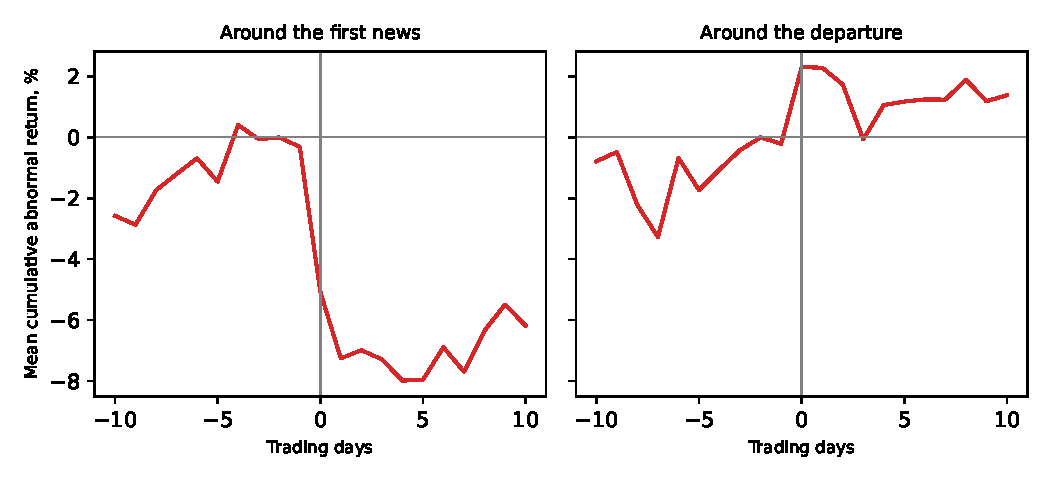
\includegraphics[width=0.85\textwidth]{fig_paths.pdf}
\caption{Mean cumulative abnormal return around the first public news, by group (constant set to zero). In two-stage cases the exit follows a median of \gap{} calendar days later.}\label{fig:paths}
\end{figure}

\begin{table}[t]\centering\scriptsize
\caption{The two-stage and survival cases}\label{tab:cases}
\setlength{\tabcolsep}{3pt}
\begin{tabularx}{\textwidth}{>{\raggedright\arraybackslash}p{3.4cm}>{\raggedright\arraybackslash}Xccrrr}\toprule
Firm (chief executive) & What became public first & First news & Exit & Day 0 & $[-1,+1]$ & Exit \\ \midrule
\tabin{tables/t_cases.tex}
\bottomrule\end{tabularx}
\par\medskip\footnotesize Abnormal returns in per cent: day 0 and $[-1,+1]$ around the first news, and $[-1,+1]$ around the exit. First news is the first trading day on which the news could affect the closing price; exit is the date of the announcement. The descriptions follow the sources, and several of the allegations were denied. $^\dagger$~Large estimated constant or a jump in the estimation window (Appendix~\ref{app:robust}).
\end{table}

\subsection{Founders and survival: Predictions 1, 4 and 7}

Table~\ref{tab:power} compares the chief executives and companies in the three groups. Founders accounted for three of the 66 one-stage cases, three of the eight two-stage cases and three of the five survival cases. The median chief executive had been in office for 5.2 years in the one-stage group, 8.6 years in the two-stage group and 22.7 years in the survival group, and the median company was worth \$1.9 billion, \$16.0 billion and \$71.9 billion respectively. A count of Dow Jones stories about each company in the year before the first news, a rough measure of press attention, is available for eight of the 13 public cases and is similar to the count for the one-stage cases.

Four of the five survival cases had small abnormal returns at the first news. At Whole Foods Market in 2007 it emerged that John Mackey, the co-founder, had for years posted under a pseudonym on an internet message board, praising his own company and disparaging a rival that the company was trying to buy. The Securities and Exchange Commission opened an informal inquiry and the board formed a special committee, and he remained chief executive. At Amazon in 2019 Jeff Bezos announced his divorce and, a few weeks later, accused the publisher of a tabloid newspaper of attempted blackmail; there was no allegation of misconduct at the company. At Best Buy in 2020 an anonymous letter alleged that the chief executive, Corie Barry, had had an undisclosed relationship with another executive. The audit committee reviewed the allegation, and less than three weeks later the board announced its support for her continued leadership. At Tesla in 2022 a newspaper reported an alleged affair, which was denied. In all four cases the abnormal return over the three days around the first news was between $-2$\% and $+2$\%.

The fifth survival case is Activision Blizzard. In November 2021 a newspaper reported that its chief executive, Bobby Kotick, had known for years about allegations of sexual misconduct at the company without telling the board about some of them, and that claims about his own conduct had been settled. The abnormal return over three days was $-7.9$\%. Analysts called for him to leave, and he told colleagues that he would consider leaving if he could not fix the company's problems quickly. In January 2022 the company agreed to be sold to Microsoft, and he stayed in office until the sale was completed.

\citet{borelli2021} find that accused chief executives who stay are associated with larger losses than those who leave. Three of the five survivors here were founders of very large companies, and none of the four survivors with small abnormal returns faced allegations of harassing employees.

\begin{table}[t]\centering\small
\caption{Chief executives and firms by group}\label{tab:power}
\footnotesize\setlength{\tabcolsep}{4pt}
\begin{tabular}{lrccccc}\toprule
 & Cases & Founders & Also chairs (\%) & Tenure, median & Market value, median & Dow Jones stories, \\
 & & & & (years) & (\$bn) & median (cases) \\ \midrule
\tabin{tables/t_power.tex}
\bottomrule\end{tabular}
\par\medskip\footnotesize Founders: the chief executive's ExecuComp title or the Gentry notes mention a founder; checked by hand for the two-stage and survival cases. Tenure and chair status come from ExecuComp and market value from Compustat, in each case for the fiscal year before the first news. Dow Jones stories: stories about the company in RavenPack's event categories from 365 to 30 days before the first news, available where the company was included in that data pull.
\end{table}

\section{Implications for investors, boards and risk managers}

For investors, the largest abnormal returns in the two-stage cases and at Nvidia followed the first public sign that the board was involved, and the abnormal return at the departure shows whether the market regarded the chief executive as a liability or an asset by then. At Nvidia much of the price movement took place before the open and after the close: on the morning of the resignation, the price before the open was well below the level that regular trading reached within an hour.

For boards, an investigation completed before any announcement presents the market with a decision in one step, and an investigation announced while it is under way is followed by a larger abnormal return at the first news. In the sample, the scandals that became public before a decision involved founders and large companies more often than the scandals that were announced together with the departure.

For risk managers, the two-stage cases and Nvidia give a range for the abnormal return of a large company run by its founder when the board's involvement first becomes public: from a few per cent to a fifth of the company's value. The abnormal return at the board's decision was smaller and had either sign.

\bibliographystyle{plainnat}
\bibliography{refs}

\appendix
\section{Coding and hand checks}\label{app:coding}

\noindent The departures with Gentry et al.\ code 4 are classified from the database's notes as personal conduct, corporate wrongdoing, or other or unclear. The candidate episodes from RavenPack are coded from their headlines in the first 30 days:
\begin{itemize}\itemsep0pt
\item P1: a serious allegation about the personal conduct of the sitting chief executive, meaning conduct outside the job at the company: a relationship or sexual conduct, harassment, a crime or personal legal charge (including trading in another company's shares), dishonesty about the chief executive's own record, personal dealings with the company or misuse of its money, or a board investigation of such conduct;
\item P2: a gaffe or controversy over the chief executive's own words;
\item W: the chief executive's conduct in running the company, including accounting fraud, conflicts of interest in a sale of the company, and trading in or statements about the company's own securities;
\item F: a legal or regulatory problem of the company that names the chief executive only as its head;
\item H: health; U: unclear; N: not a scandal; DUP: duplicate.
\end{itemize}
The sample uses the P1 episodes and the departures over personal conduct, and the same line between personal conduct and conduct in running the company is applied to both sources. Four episodes first coded P1 were recoded W because they concern trading in, or statements about, the company's own securities (Swift Transportation 2004, Eastman Kodak 2021, Tesla 2018) or the chief executive's role in the company's research (Citigroup 2002). For the same reason, three Gentry departures over trading in the company's own shares (Swift Transportation 2005, Fremont General 2006 and The Children's Place 2007) count as corporate wrongdoing, and Papa John's in 2017, a departure after public remarks, counts as other. Jabil in 2024 is coded U: its chief executive was placed on leave pending an investigation ``related to corporate policies'' and left a month later, and the company did not say what the conduct was.

The dates of the two-stage and survival cases were checked against filings with the Securities and Exchange Commission, company announcements and news reports. Two first-news dates were moved earlier as a result. Chesapeake Energy's was moved to 18 April 2012, the day of the news agency report on the chief executive's personal loans; the shareholder lawsuit came two days later. Whole Foods Market's was moved to 12 July 2007, the first trading day after the report on the chief executive's online posts; the episode found by the search began with a later feature article. For Wynn Resorts, CBS and WWE the first news is the first Dow Jones story about the allegation, which came before the departure recorded in the Gentry data. Exit dates were corrected for Chesapeake (whose chief executive's retirement was announced after the close on 29 January 2013) and Intel (21 June 2018), and duplicate records were removed. The coding files hold only case identifiers and codes, because the Dow Jones headlines may not be redistributed.

\section{Robustness}\label{app:robust}

Table~\ref{tab:robust} compares the main specification with the full market model and with market-adjusted returns, and it reports, for the small groups, the range of the group mean when each case is dropped in turn. Across the three models, the estimates at the first news and at the departure differ by no more than 0.3 percentage points. Among the two-stage and survival cases, AdaptHealth and Whole Foods have large estimated constants, and their 60-day returns depend on the model. The survivors' mean return over the 60 days after the first news is $+8.4$\%, with Activision Blizzard, whose agreed sale to Microsoft was announced within that window, and Whole Foods as the largest contributions; the median is $-2.4$\%.

\begin{table}[!ht]\centering\small
\caption{Three-day abnormal returns under three models (\%)}\label{tab:robust}
\footnotesize\setlength{\tabcolsep}{3pt}
\begin{tabular}{>{\raggedright\arraybackslash}p{3.3cm}ccccccc}\toprule
 & \multicolumn{4}{c}{First news} & \multicolumn{3}{c}{Exit} \\ \cmidrule(lr){2-5}\cmidrule(lr){6-8}
 & Main & Full model & Market-adj. & Leave one out & Main & Full model & Market-adj. \\ \midrule
\tabin{tables/t_robust.tex}
\bottomrule\end{tabular}
\par\medskip\footnotesize Main: market model with the constant set to zero. Full model: estimated constant and slope. Market-adjusted: the share's return minus the market return. Leave one out: the range of the group mean when each case in turn is dropped.
\end{table}

\end{document}
